\documentclass[ ]{article}
\usepackage{pythonhighlight}
\usepackage[margin=0.5in]{geometry}
\usepackage{color, colortbl}
\usepackage{xcolor}
\usepackage{graphicx}
\usepackage{caption}


\definecolor{Gray}{gray}{0.9}
\definecolor{DarkGray}{gray}{0.5}
\definecolor{LightCyan}{rgb}{0.88,1,1}
\definecolor{yellow}{rgb}{1,1,0}

\begin{document}

\noindent
{\LARGE \textbf{Partie Appliquée}}
\vspace{5 mm}

\noindent
Dans cette section, nous allons tester et comparer les différents algorithmes de Kmeans, Kmeans++ et Kmeans++ semi-supervisées sur un jeu de données clients. Nos mesures de performances sont le coût tel qu'estimé par la fonction potentiel, ainsi que la durée d'exécution de l'algorithme.

\vspace{10 mm}

\noindent
{\Large \textbf{La Base de Données}}
\vspace{5 mm}

\noindent
La base de données contient 60366 observations (clients) et 39 variables quantitatives et qualitatives. Tous les clients sont anonymisés se qui limitera l'interprétation de l'analyse.

\noindent
Nous commençons par analyser la base de données. Ci-dessous, nous affichons la statistique d'une partie de nos données. 
\begin{center}
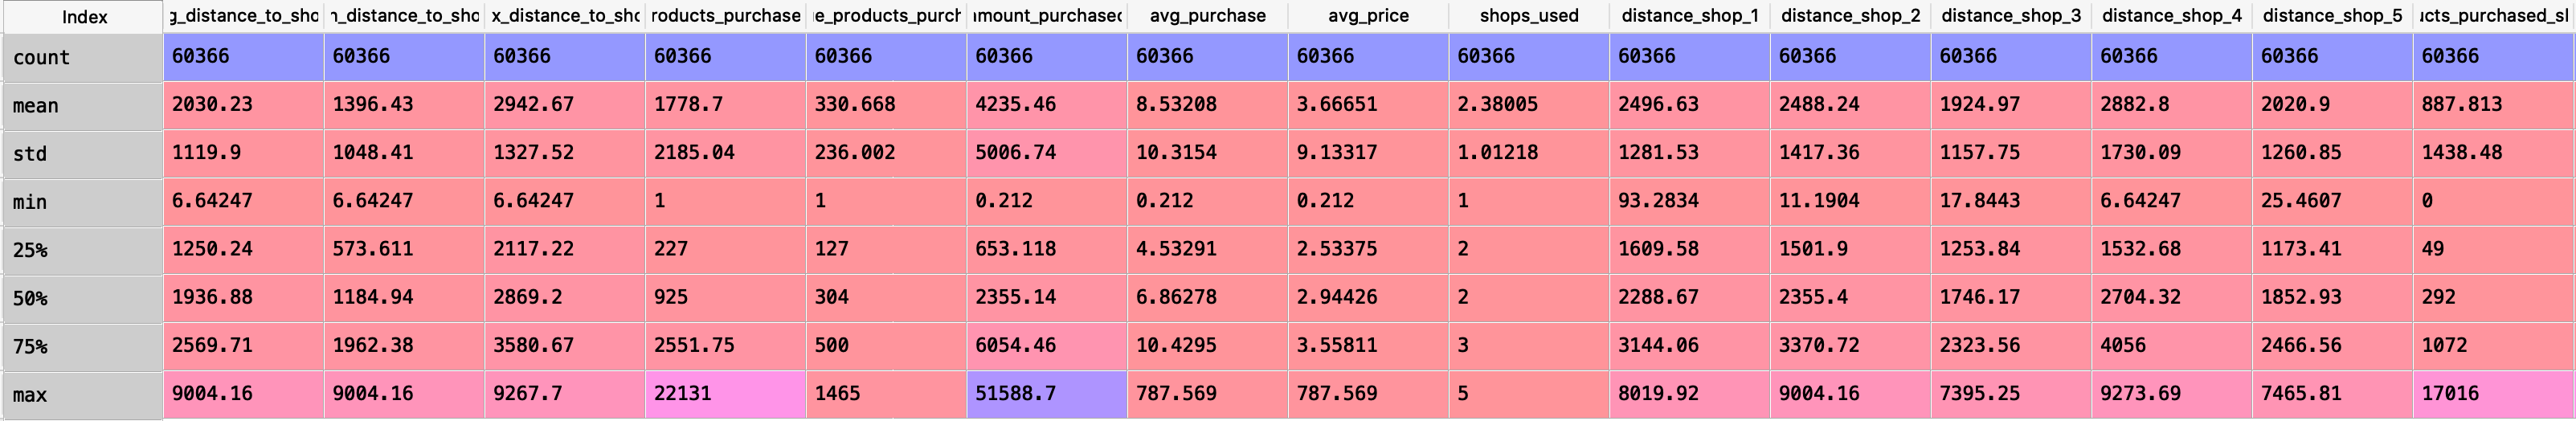
\includegraphics[scale=0.35]{summary.png}
\end{center}

\noindent
Nous voyons qu'il existe une seule variable qualitative, la variable 'shops used', les autres étant toutes des variables quantitatives continues. Nous remarquons aussi que toutes les variables quantitatives affichent de grandes dispersions. Par exemple, en regardant le nombre de produits achetés, nous voyons que certains clients achètent très peu, soit 1 seul article, tandis que d'autres achètent jusqu'à 22 131 articles, la moyenne étant 2552.75. Ce type d'observation nous permettra de mieux interpréter les clusters proposés par les différentes versions des k-means.

\noindent
Une Analyse en Composantes Principales est implémentée afin de mieux regrouper et comprendre les variables quantitatives. Le choix du nombre de composantes principales est basé sur le pourcentage de la variance expliquée ainsi que par la méthode du coude (une baisse soudaine de la variance expliquée entre deux composantes).

\begin{center}
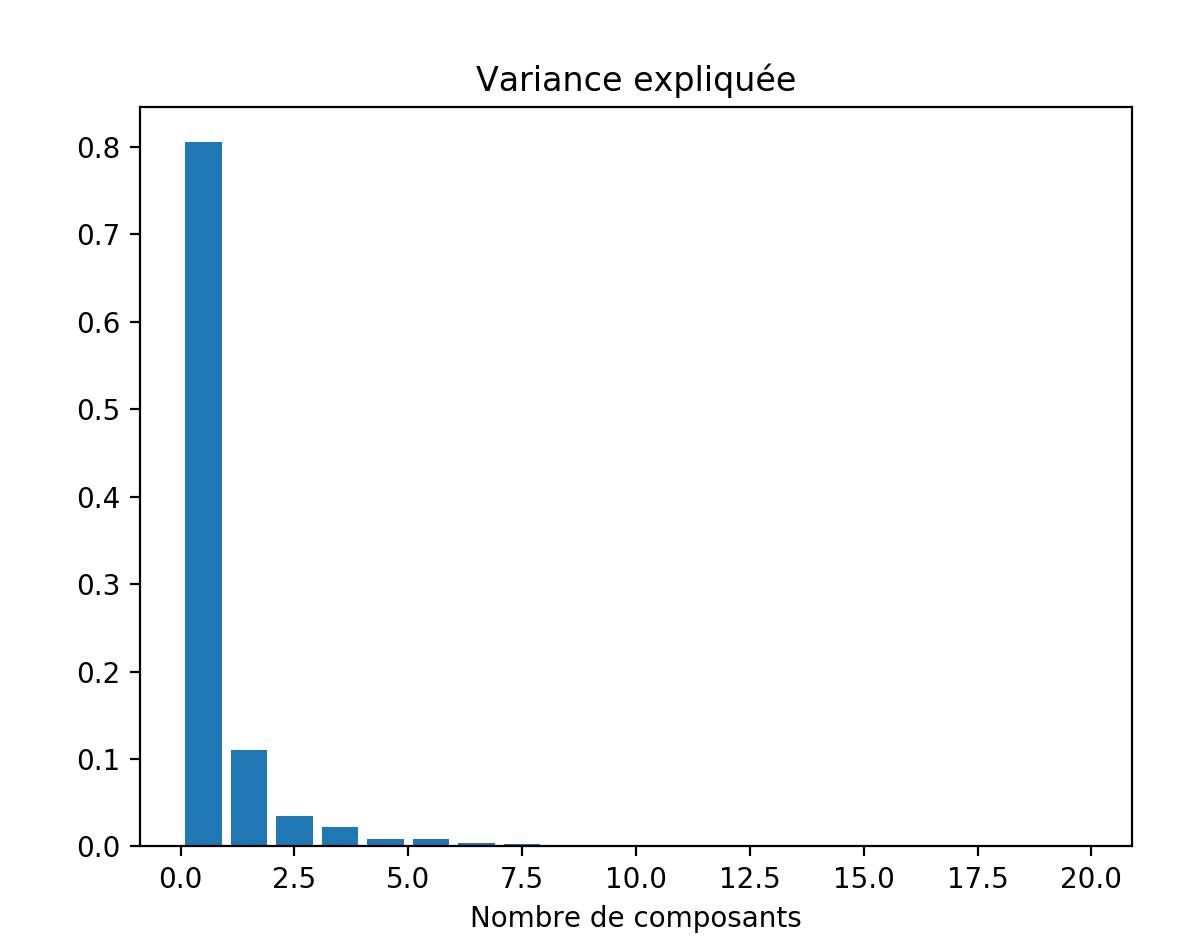
\includegraphics[scale=0.50]{variance_explique.png}
\end{center}

\noindent
Nous voyons ici que les premières composantes principales expliquent une bonne partie de l'inertie, soit plus de 80\% de la variance, et ainsi nous nous baserons uniquement sur l'analyse en composantes principales sur 2 et 3 dimensions. 

\noindent
Sur un plan 1-2 nous obtenons le graphique tel qu'affiché ci-dessous:

AFFICHER ACP SUR LE PLAN 1-2 (DIMENSION 2)

AFFICHER ACP SUR 3 DIMENSIONS



\vspace{5 mm}
\noindent
\begin{large}
\textbf{Choix du nombre de clusters}
\end{large}

\noindent
La méthode K-means est une méthode d'apprentissage non-supervisée. Lors de son application les données sont séparées en plusieurs classes prédéterminés de façon que les individus ayant le plus de similarité. C’est ainsi qu’une des tâches clefs est de trouver le nombre approprié de classes, k. Il existe plusieurs techniques pour déterminer le nombre de classes. Nous discuterons que des cas les plus connus : 
\begin{description}
  \item 1. Méthode du pouce:
  
  Cette méthode est une méthode approximative où le nombre de classes, k est déterminé par : 
$ k \approx \sqrt{n/2}$

    \item 2. L'indice de qualité:
    
	Afin d’évaluer la qualité de la classification, les indices inertiels , soient l’inertie intra-classes et l’inertie l’inter-classes sont souvent utilisés. L’inertie intra-classes ‘mesure le degré d’homogénéité entre les objets appartenant à la même classe‘ tandis que l’inertie inter-classes ‘mesure le degré d’hétérogénéité entre les classes.’
Il existe plusieurs indices de qualité, par exemple l’indice de Dunn, l’indice de Calinski et Harabasz (CH) ou encore l’indice de Silhouette. 
Le premier calcule la distance minimale inter-classes et ainsi plus cette distance est grande, meilleur sera la classification. 

Introduit par Kauffman et Rousseew, l’indice de Silhouette nous donne une représentation visuelle de la distance entre un point d’une classe avec les points des classes voisines. Plus le coefficient ainsi calculé est proche de 1, plus la distance avec les classes voisines (inertie inter) est grande. Ceci représente le nombre de classes optimale. À l’inverse, un coefficient proche de -1 nous indique une mauvaise classification de l’observation.


		\item 3. Méthode du coude:
		
  La méthode du coude est une technique visuelle très connue. L’idée derrière cette technique est d’implémenter la méthode K-means en parcourant k valeurs. À chacune des k valeurs, la somme des erreurs au carré est calculée et est affiché sur un graphique, nous permettant à mieux visualiser les résultats. L’objectif est de choisir la valeur k (qui sera le nombre de classes) créant un effet de ‘coude’, c’est-à-dire provoquant une baisse plus conséquente, plus soudaine de la somme des erreurs au carré. Nous disons ceci en gardant en tête que la somme des erreurs aura toujours tendance à baisser, plus la valeur de k est grande. 
  
 	 \item 4. La validation croisée:
 	 
La validation croisée regarde la stabilité des classes. Les données sont séparées en au moins deux parties. La première est utilisée pour former les classes tandis que la deuxième sert de validation. Lorsque nous parlons de stabilité, nous parlons de la fréquence à laquelle des classes similaires sont formées lorsque plusieurs itérations sont effectuées. Ainsi une plus grosse fréquence de l’apparition de mêmes classes équivaut à une plus grosse stabilité de ces classes.
 	 
\end{description}

\noindent
Dans le cadre de notre étude, nous choisissons de travailler avec la méthode du coude, une méthode que nous appliquons sur la méthode de kmeans++. Cette méthode est d'ailleurs comparée avec celle de sklearn afin de déterminer l'exactitude de l'algorithme utilisé. Le graphique ci-dessous affiche la répartition des sommes des erreurs au carré à la fois pour notre méthode, dite la méthode manuelle, ainsi que la méthode proposé par sklearn. Nous voyons une baisse plus soudaine lorsque nous avons 5 clusters. Ce sera ainsi le choix du nombre de clusters utilisé lors de l'application des algorithmes de clustering.

\begin{center}
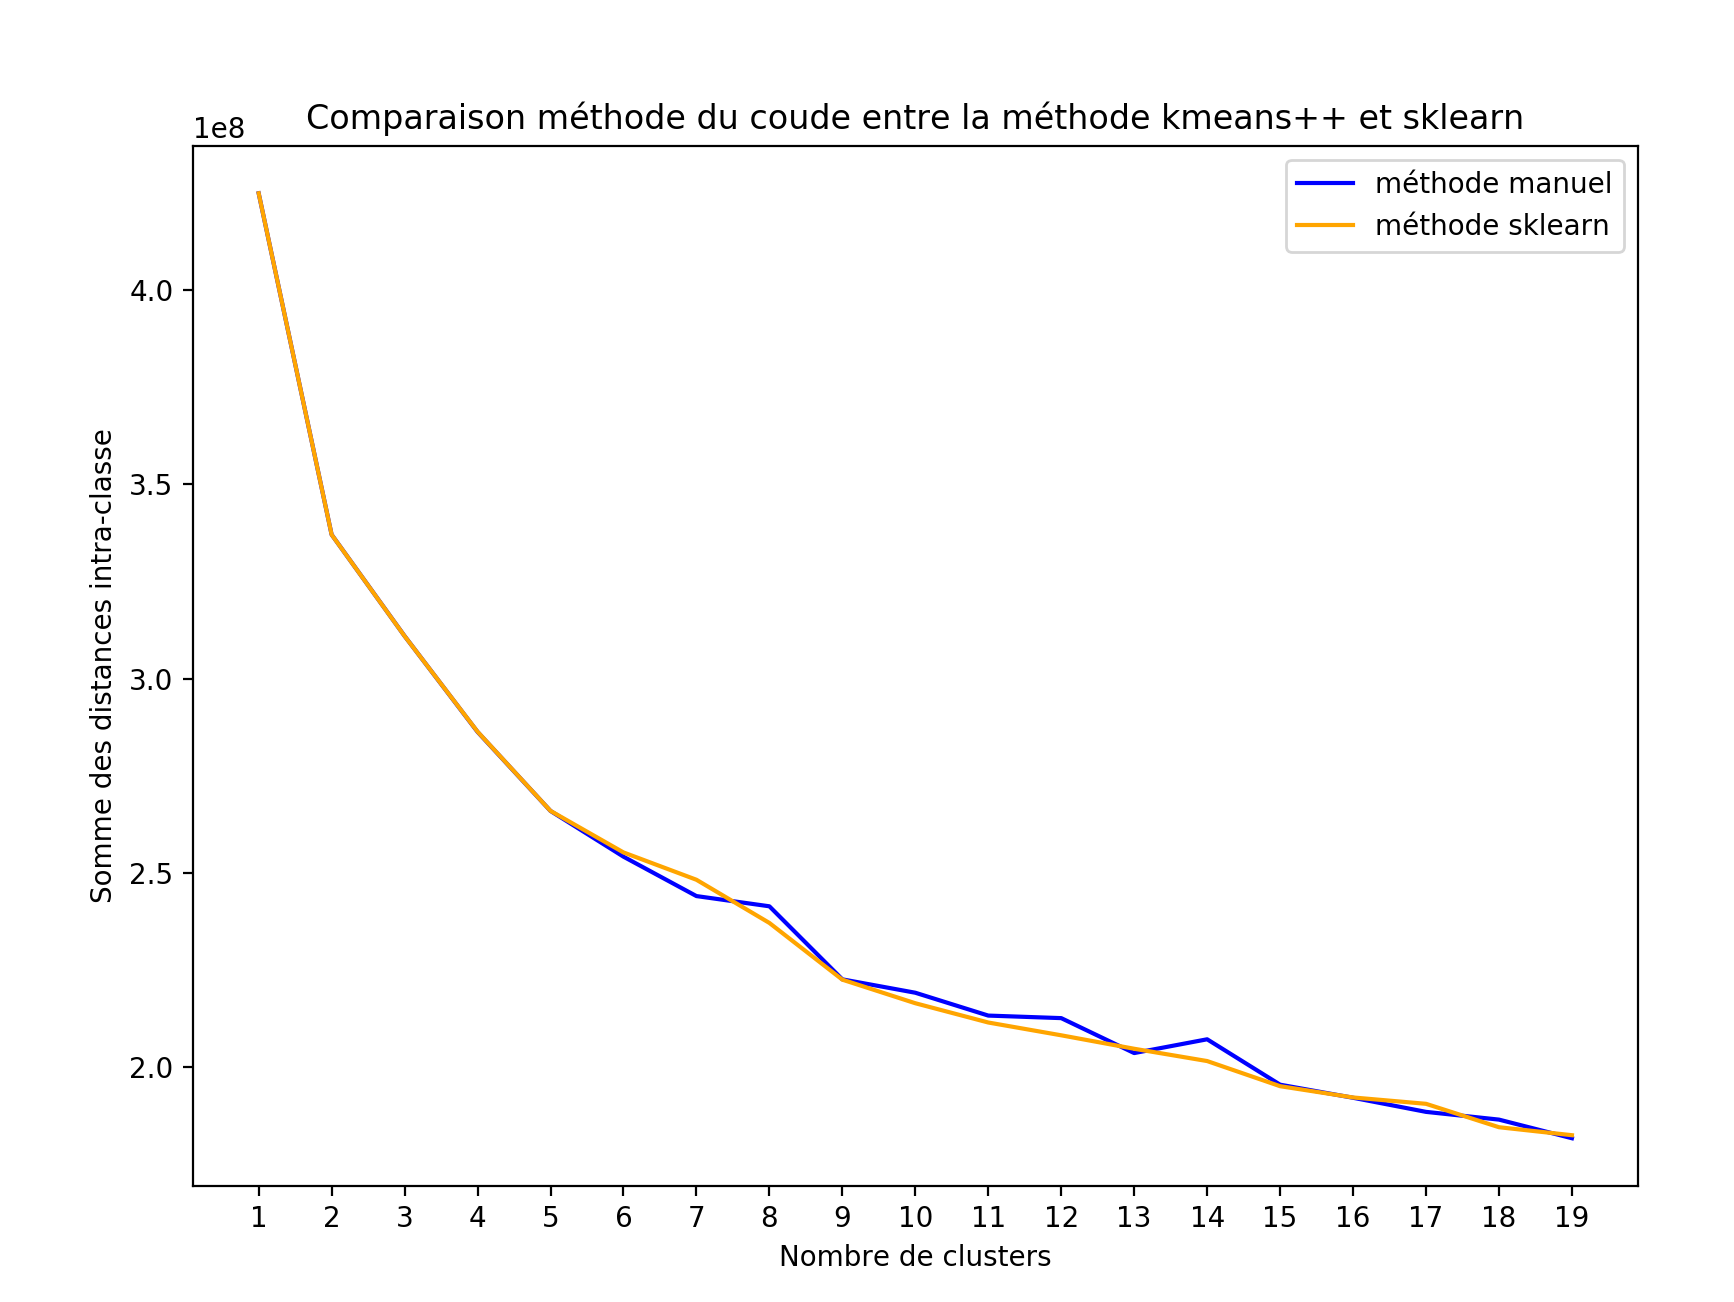
\includegraphics[scale=0.50]{Comparaison_elbow.png}
\end{center}

\begin{center}
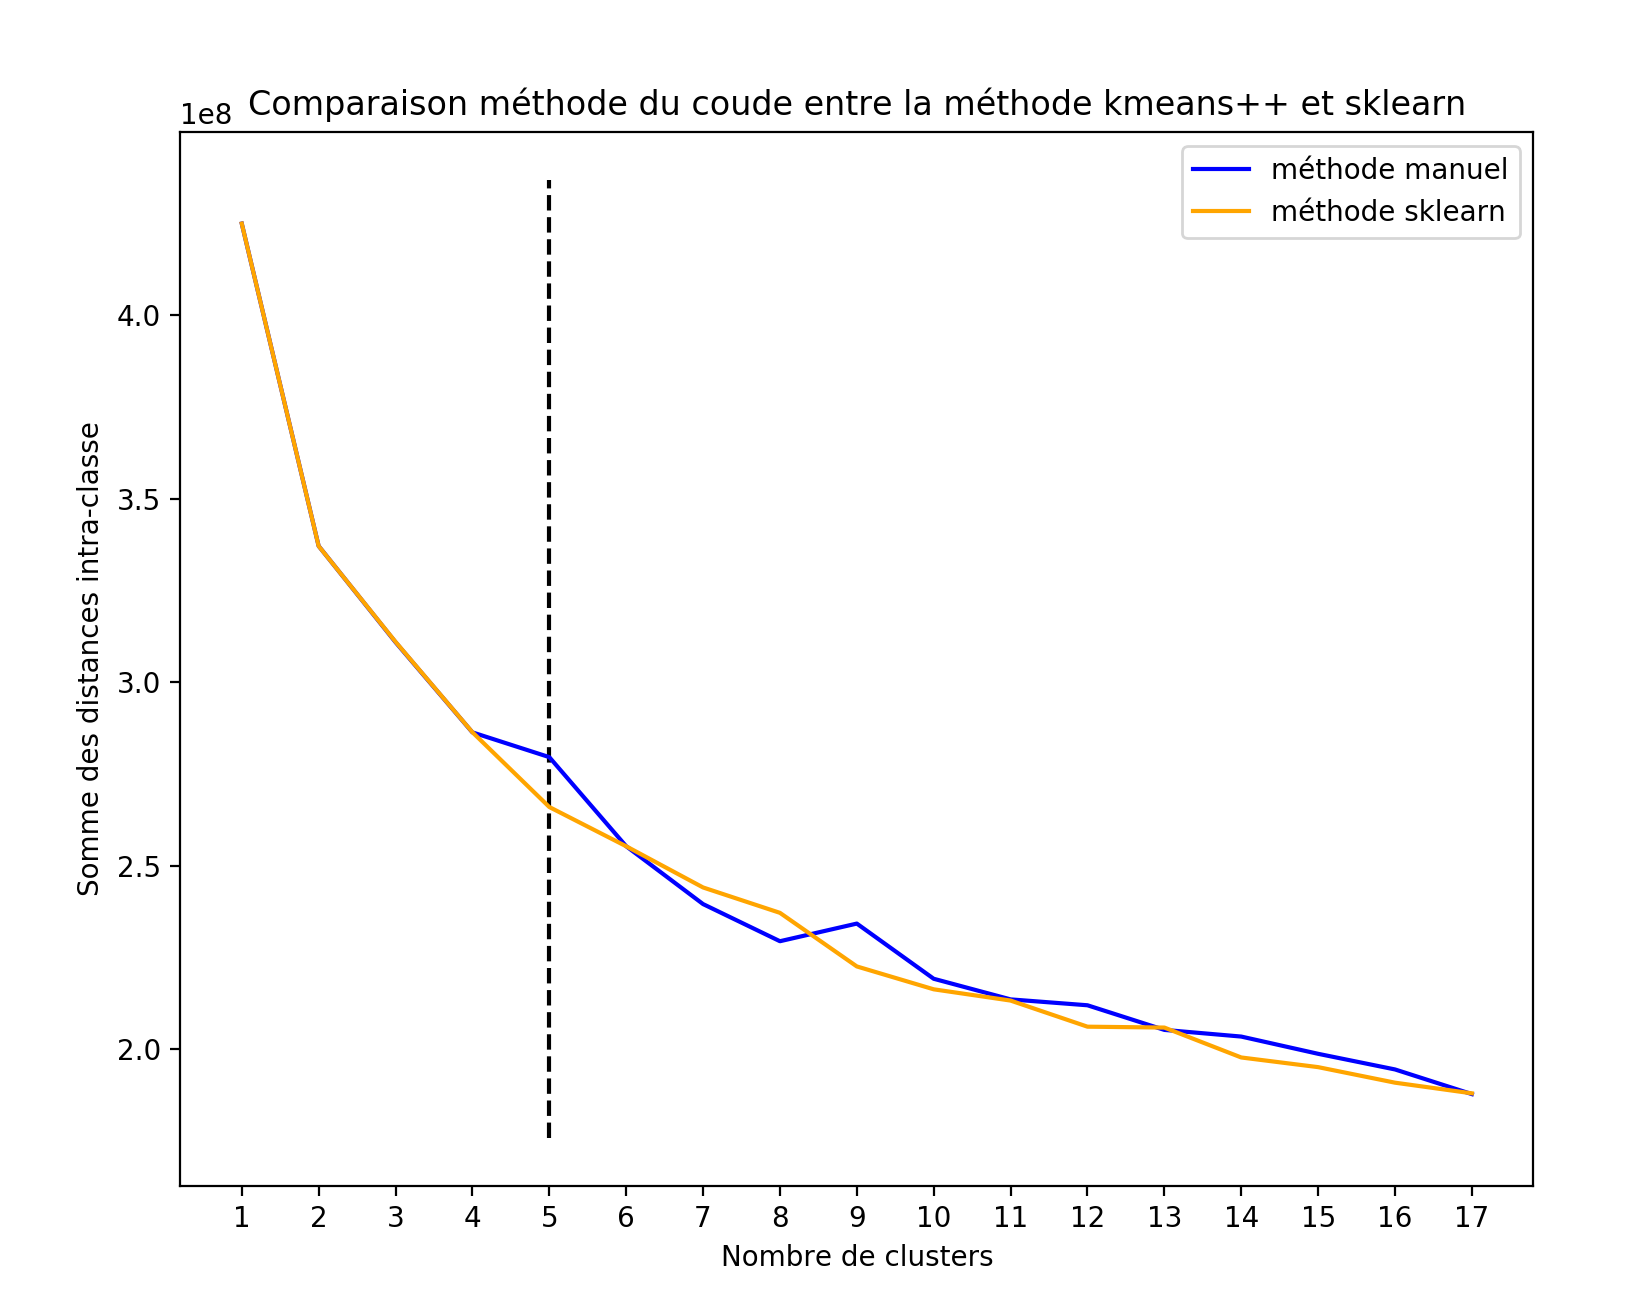
\includegraphics[scale=0.50]{Comparison_elbow2.png}
\end{center}

\vspace{5 mm}
\noindent
\begin{large}
\textbf{Observations et Résultats}
\end{large}

\noindent
Dans cette section nous cherchons à présenter les résultats obtenus par les algorithmes kmeans, kmeans++ et kmeans++ semi supervisées. De plus ce dernier a été analysé plus en détails afin d'afficher l'impact des différents pourcentages de données labellisés. Comme pour l'ACP la variable qualitative a été écartée de notre analyse.
6 essaies ont été effectués afin d'évaluer le temps d'exécution des algorithmes (en secondes). La moyenne des distances intra-classes a été obtenu en se basant sur 100 simulations. Le nombre de clusters, déterminé en utilisant la méthode du coude, est 5.

\noindent
Le graphique ci-dessous affiche les 5 clusters ainsi que leurs centres, tel que proposé par l'algorithme kmeans++ semi-supervisée.

\begin{center}
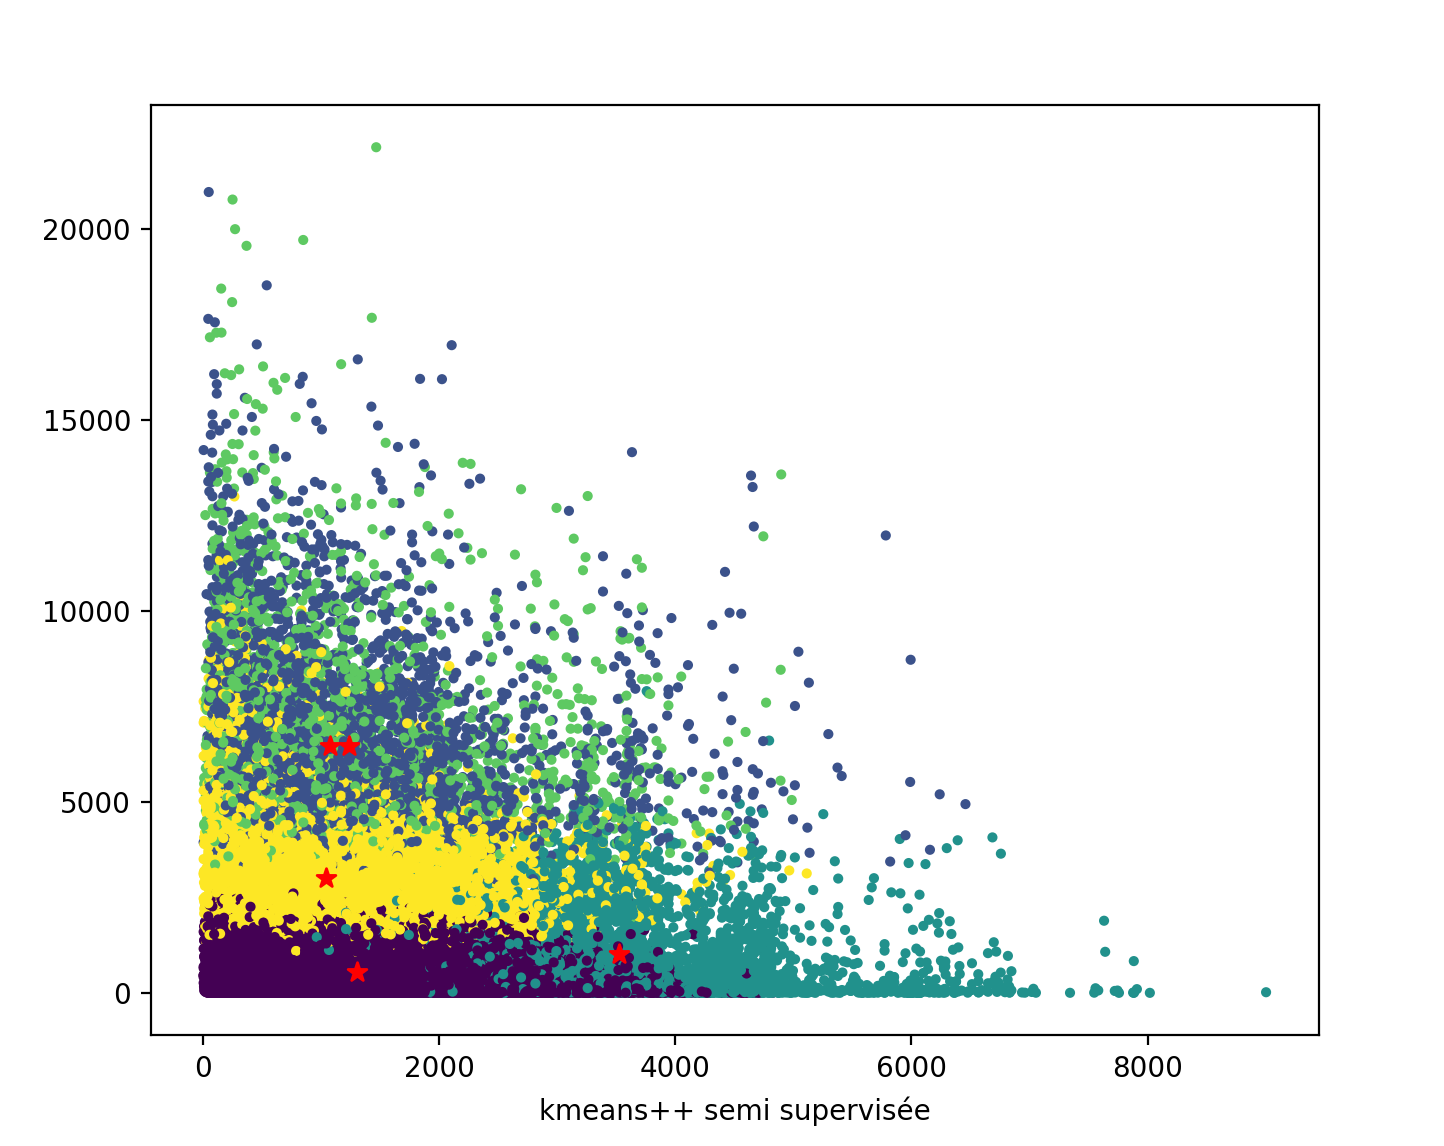
\includegraphics[scale=0.50]{kmeanspp_ss.png}
\end{center}


\vspace{10 mm}
\noindent
Les tableaux ci-dessous affichent les résultats obtenus pour les différents algorithmes.

\begin{table}[ht]
\centering

\vspace{10 mm}
\caption{\textbf{Résultats en utilisant kmeans}} 

\begin{tabular}{c|c|c|c}
\hline
\rowcolor{Gray}
Temps d'exécution Minimum & Temps d'exécution Maximum & Temps d'exécution Moyen & Moyenne des distances intra-classe \\
\hline
0.867459&4.278867& 1.867284& \cellcolor{LightCyan}267024131.97\\

\end{tabular}

\centering

\vspace{10 mm}
\caption{\textbf{Résultats en utilisant kmeans++}} 

\begin{tabular}{c|c|c|c}
\hline
\rowcolor{Gray}
Temps d'exécution Minimum & Temps d'exécution Maximum & Temps d'exécution Moyen & Moyenne des distances intra-classe \\
\hline
0.952380&1.963426& 1.603216& \cellcolor{LightCyan}269311160.94\\

\end{tabular}

\centering

\vspace{10 mm}
\caption{\textbf{Résultats en utilisant kmeans++ semi-supervisées avec 60\% de données labellisées}} 

\begin{tabular}{c|c|c|c}
\hline
\rowcolor{Gray}
Temps d'exécution Minimum & Temps d'exécution Maximum & Temps d'exécution Moyen & Moyenne des distances intra-classe \\
\hline
0.386259&0.616933& 0.481936& \cellcolor{LightCyan}265971783.28\\
\end{tabular}

\end{table}

\vspace{10 mm}


\noindent 
Tel que prévu la durée d'exécution moyenne de l'algorithme de kmeans est plus longue que celle du kmeans++ et du kmeans++ semi-supervisée (avec 60\% de données labellisées). Cette dernière est d'ailleurs en moyenne > 3 fois plus rapide que le kmeans ou le kmeans++. Au niveau du coût de la fonction nous voyons que le kmeans ++ semi supervisée affiche à nouveau le meilleur résultat (avec la plus petite distance moyenne intra-classes sur 100 simulations). Il est toutefois étonnant de voir que la distance intra-classe moyenne lorsque kmeans est utilisé est plus petite que celle du kmeans++. 


\noindent






\vspace{5mm}
\noindent

\begin{description}
  \item 1. 
  \item 2. 
  \item 3. 
  \item 4.
\end{description}




\end{document}
